\chapter{The Analysis Pipeline}
\label{ch:analysis_pipeline}

\section{Overview}
\label{sec:pipeline_overview}

The analysis system is modeled as a composition of three sequential
transformations, each operating on well-defined input and output
domains. Let $\mathcal{L}$ be the set of supported languages,
$\mathcal{W}$ the domain of a Workspace (a collection of source files
$\mathcal{S}_{code}$), and $\mathcal{D}_{IR}$ the domain of the
Intermediate Representation defined in Chapter
\ref{ch:ir_formalization}. The complete analysis function $\Phi$ is defined as:
$$\Phi : \mathcal{W} \to \mathcal{G} \qquad \Phi = \gamma \circ R \circ E_w$$

The pipeline is illustrated in Figure \ref{fig:analysis_pipeline}.
Each phase receives the output of its predecessor and produces a
strictly richer representation of the codebase.

\begin{figure}[htpb]
  \centering
  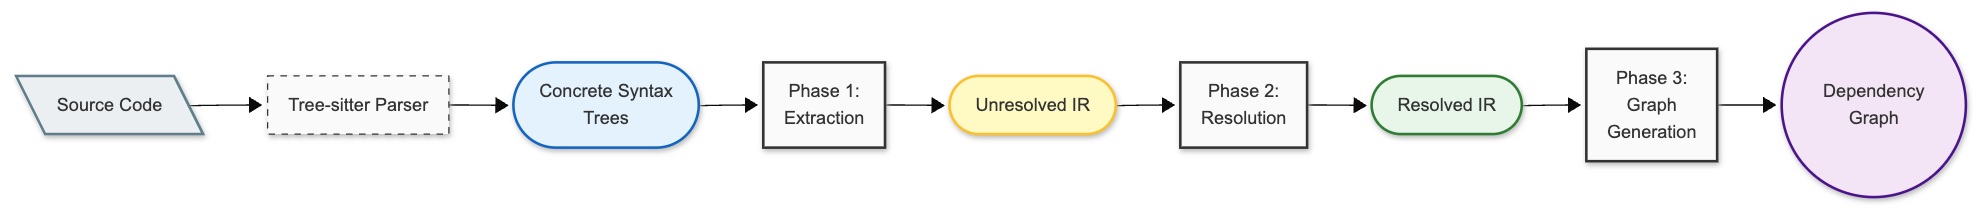
\includegraphics[width=\textwidth]{images/analysis_pipeline.png}
  \caption{Overview of the three-phase analysis pipeline, from source
  code to dependency graph.}
  \label{fig:analysis_pipeline}
\end{figure}

A fundamental design property of this decomposition is the separation
between language-dependent and language-independent logic. Phase 1 is
the only phase that interacts with language-specific syntax; Phases 2
and 3 operate entirely on the language-agnostic IR, ensuring that the
core analytical logic is shared across all supported languages.

\section{Phase 1: Syntactic Extraction ($E_w$)}
\label{sec:phase1_overview}

$$E_w : \mathcal{W} \to \vec{\mathcal{M}}$$

The extraction phase transforms source code into the Intermediate
Representation. For each source file in the workspace, a Tree-sitter
parser \cite{TODO:tree_sitter} generates a Concrete Syntax Tree
(CST), which is then traversed by a set of heuristic classifiers and
parsers to identify and extract the relevant software components
(modules, structured types, functions, fields, imports, and
implementation blocks).

\subsection{Input}

The input is a \textbf{Workspace} $\mathcal{W}$: a directory tree
containing source files in one or more of the supported languages (C,
C++, Java, Python, Rust). Each file is independently parsed and extracted.

\subsection{Process}

The extraction operates through four logical layers:

\begin{enumerate}
  \item \textbf{Parsing}: Tree-sitter generates a CST for each source
    file, preserving every token of the original code.
  \item \textbf{Classification}: Heuristic predicates inspect CST
    node kinds (e.g., \texttt{struct\_item},
    \texttt{function\_definition}, \texttt{class\_declaration}) using
    string-based pattern matching to determine the role of each node.
    This approach exploits the structural similarity of Tree-sitter
    grammars across languages to avoid maintaining per-language rule sets.
  \item \textbf{Structural Parsing}: Classified nodes are transformed
    into IR components by extracting their constituent parts (names,
    fields, methods, parameters, return types, super-types, annotations).
  \item \textbf{Body Extraction}: Function bodies are analyzed to
    extract behavioral dependencies (function calls, type
    instantiations, field accesses, type casts) and local variable
    declarations, organized into a recursive \texttt{Block} structure
    that mirrors the lexical scope hierarchy of the source code.
\end{enumerate}

After individual file extraction, a \textbf{Module Grouping Strategy}
organizes the extracted modules into a hierarchical tree that
reflects the project's namespace conventions. Different strategies
are applied depending on the language: directory-based namespacing
(Python, Rust), package declarations (Java), explicit namespace
blocks (C++), or a flat fallback (C). For C++, an additional
\textbf{out-of-line method linking} step associates method
definitions written in \texttt{.cpp} files with their class
declarations in \texttt{.hpp} headers.

\subsection{Output}

The output is a forest of \textbf{Module trees} $\vec{\mathcal{M}}$,
unified across all files in the workspace. Each module contains its
structured types, free functions, imports, implementation blocks,
type aliases, and free variables. All type references ($\tau$) at
this stage are in the \texttt{Unresolved} state: they carry the
symbolic name extracted from the source code but have not yet been
linked to their target component.

\subsection{Key Properties}
\begin{itemize}
  \item This is the \textbf{only language-dependent} phase. The
    heuristic classifiers and extractors are the sole components that
    interact with language-specific CST node kinds.
  \item Each file is extracted \textbf{independently}. Cross-file
    dependencies are not resolved in this phase.
  \item The output IR is \textbf{structurally complete} but
    \textbf{semantically unresolved}: the topology of the codebase
    (what components exist and what they contain) is fully captured,
    but the targets of type references are not yet known.
\end{itemize}

The detailed implementation of this phase, including the heuristic
classification system, the extraction algorithms, and the module
grouping strategies, is presented in Chapter \ref{ch:extraction}.

\section{Phase 2: Name Resolution ($R$)}
\label{sec:phase2_overview}

$$R : \vec{\mathcal{M}} \to \vec{\mathcal{M}}$$

The name resolution phase transforms the symbolic type references
produced by extraction into resolved semantic pointers. This is the
phase that connects the isolated components into a coherent
dependency network by determining, for each type reference, which
component in the workspace it refers to.

\subsection{Input}

The input is the unified forest of module trees $\vec{\mathcal{M}}$
produced by Phase 1, where all type references are in the
\texttt{Unresolved} state.

\subsection{Process}

The resolution is decomposed into two algebraic sub-phases:

\begin{enumerate}
  \item \textbf{Query Building} ($R_{build}$): The module hierarchy
    is traversed with an ephemeral \textit{Symbol Stack} ($\rho$)
    that tracks local variable bindings. Each \texttt{Unresolved}
    type reference is replaced by an algebraic \textit{Resolution
    Query} ($\mathcal{Q}$) composed of three primitives:
    \begin{itemize}
      \item \texttt{Find($s$)}: Ascending scope search for identifier $s$.
      \item \texttt{Extract($q$, $s$)}: Structural member access on
        the result of sub-query $q$.
      \item \texttt{Call($q$)}: Return-type extraction after
        evaluating sub-query $q$ as a callable.
    \end{itemize}
    The Symbol Stack enables local variable substitution: when a
    reference such as \texttt{x.method()} is encountered, the stack
    replaces \texttt{x} with its declared type, transforming the
    reference into a query that can be resolved globally.

  \item \textbf{Query Execution} ($R_{exec}$): A global \textit{Scope
    Tree} ($\mathcal{E}$) is constructed from the entire workspace
    using an arena allocator. Each query expression is then evaluated
    against this tree using \textit{Lexical Scope Climbing}: starting
    from the scope where the reference was declared, the algorithm
    ascends the parent chain, checking local symbols, imports, and
    inherited members, until the target is found or the root is reached.
\end{enumerate}

The resolution is parameterized by a per-language
\textbf{configuration} ($\mathcal{K}_{cfg}$) that controls behaviors
such as transitive import resolution, implicit self/this parameter
injection, and Deref coercion handling.

\subsection{Output}

The output is the same forest of module trees $\vec{\mathcal{M}}$,
but with all type references transformed into one of four terminal states:

\begin{itemize}
  \item \texttt{Resolved($\pi$)}: The reference was successfully
    linked to a component within the workspace, identified by its
    absolute qualified name $\pi$.
  \item \texttt{External($\pi$)}: The reference points to a component
    outside the analyzed workspace (e.g., standard library types,
    third-party dependencies).
  \item \texttt{Primitive($s$)}: The reference is a built-in
    primitive type (e.g., \texttt{int}, \texttt{bool}, \texttt{String}).
  \item \texttt{Failed($\pi$)}: The resolution was unsuccessful (the
    target could not be found in any accessible scope).
\end{itemize}

\subsection{Key Properties}
\begin{itemize}
  \item This phase is \textbf{completely language-independent}. The
    resolution algorithm operates solely on the IR, with
    language-specific behavior controlled by configuration flags.
  \item The resolution is \textbf{workspace-global}: because the
    Scope Tree is built from all files simultaneously, cross-file
    dependencies are resolved transparently.
  \item The Execution Context ($\Gamma = \langle \mathcal{E},
    \mathcal{PR}, \mathcal{K}_{cfg} \rangle$) is \textbf{immutable}
    during query evaluation, guaranteeing deterministic results
    independent of evaluation order.
\end{itemize}

The detailed implementation of this phase, including the query
algebra, the Scope Tree construction, the lexical climbing algorithm,
and the inheritance resolution mechanism, is presented in Chapter
\ref{ch:name_resolution}.

\section{Phase 3: Graph Construction ($\gamma$)}
\label{sec:phase3_overview}

$$\gamma : \vec{\mathcal{M}} \to \mathcal{G}$$

The graph construction phase projects the resolved IR into a flat
directed dependency graph $\mathcal{G} = (V, E)$ suitable for
architectural analysis and visualization.

\subsection{Input}

The input is the resolved forest of module trees $\vec{\mathcal{M}}$
produced by Phase 2, where type references are in their terminal states.

\subsection{Process}

The construction proceeds in two steps:

\begin{enumerate}
  \item \textbf{Node Flattening}: The hierarchical module tree is
    recursively traversed, and every component (module, structured
    type, function, field, type alias) is extracted into a flat
    vector of vertices $V$. Each vertex receives a globally unique
    qualified name computed by prepending all ancestor module names.
    Additionally, implicit nodes are synthesized for primitive types
    and external dependencies that are referenced by edges but not
    declared in the workspace.
  \item \textbf{Edge Generation}: The module tree is traversed a
    second time, inspecting every resolved type reference to emit
    directed edges. The system defines 15 distinct edge kinds
    organized into five categories: structural (containment and
    nesting), inheritance, type-level (field types, parameter types,
    return types), behavioral (calls, instantiations, field
    accesses), and auxiliary (imports, casts, annotations). After
    generation, edges are deduplicated to prevent inflated coupling metrics.
\end{enumerate}

The graph is exported in two formats: a raw JSON serialization of the
full \texttt{DependencyGraph} structure, and a
Cytoscape.js-compatible format \cite{TODO:cytoscape_js} where
structural containment is encoded as compound node nesting rather
than explicit edges.

\subsection{Output}

The output is a \textbf{Dependency Graph} $\mathcal{G} = (V, E)$:
\begin{itemize}
  \item $V$: A flat set of vertices, each identified by its absolute
    qualified name and typed by its component kind (Module, Class,
    Struct, Function, Field, etc.).
  \item $E$: A set of directed edges, each a triple $\langle
    \pi_{from}, \pi_{to}, \text{kind} \rangle$ specifying the source,
    target, and nature of the dependency.
\end{itemize}

An \texttt{AnalysisSummary} is also produced, containing aggregate
statistics (total modules, structured types, free functions, resolved
references, and failed references).

\subsection{Key Properties}
\begin{itemize}
  \item This phase is \textbf{completely language-independent}.
  \item Edges are generated \textbf{only} from resolved type
    references (\texttt{Resolved} and \texttt{External}). Failed or
    unresolved references do not produce spurious edges.
  \item The graph is \textbf{flat}: the original hierarchical nesting
    is encoded either as explicit containment edges or, in the
    Cytoscape export, as compound node parent relationships.
\end{itemize}

The detailed implementation of this phase, including the flattening
algorithm, the complete edge taxonomy, and the Cytoscape export
process, is presented in Chapter \ref{ch:graph_construction}.

\section{End-to-End Data Flow}
\label{sec:data_flow}

Table \ref{tab:pipeline_summary} summarizes the input, output, and
key characteristics of each phase.

\begin{table}[htpb]
  \centering
  \small
  \begin{tabular}{|l|l|l|l|l|}
    \hline
    \textbf{Phase} & \textbf{Input} & \textbf{Output} &
    \textbf{L-dependent?} & \textbf{Scope} \\ \hline
    1. Extraction & Source files ($\mathcal{W}$) & Unresolved IR
    ($\vec{\mathcal{M}}$) & Yes & Per-file \\ \hline
    2. Resolution & Unresolved IR ($\vec{\mathcal{M}}$) & Resolved IR
    ($\vec{\mathcal{M}}$) & No & Workspace-global \\ \hline
    3. Graph Construction & Resolved IR ($\vec{\mathcal{M}}$) &
    Dependency Graph ($\mathcal{G}$) & No & Workspace-global \\ \hline
  \end{tabular}
  \caption{Summary of the three pipeline phases: inputs, outputs,
  language dependency, and operational scope.}
  \label{tab:pipeline_summary}
\end{table}

This pipeline design ensures that:
\begin{enumerate}
  \item Each phase is a \textbf{pure function} operating on
    well-typed domains. The composition $\Phi = \gamma \circ R \circ
    E_w$ is itself well-typed.
  \item Adding support for a new language requires implementing
    \textbf{only} the extraction heuristics (Phase 1). Phases 2 and 3
    are entirely reused.
  \item The pipeline \textbf{terminates} for all valid inputs: the
    CST traversal is bounded by the finite tree depth, the scope
    climbing is bounded by the finite scope depth, and cycle
    detection prevents infinite loops in inheritance resolution.
\end{enumerate}
